\documentclass[IDF.tex]{subfiles}
\newpage
\begin{document}

\section{Inverted File Project}
The goal of this part of the project was to build an inverted file using a MapReduce job that computed the term-frequency (tf), inverse-document-frequency (idf) and the tf-idf parameters for words within a given text blob. The testing was done using the 'summary' sections from the \textit{movies.xml} database that we have used from earlier assignments. 

\subsection{Major Components}

The Java program is built as a command-line tool and takes 2 or more arguments. The first to second last arguments are the input files on which the MapReduce operations are performed. The input files need to be in XML format and should contain a 'summary' tag else the tf-idf calculations will be skipped. Listed below are the major components for this application:
\begin{itemize}
\item com.hadoop.movies.ReadMovieXML - This class parses the 'summary' tags from input XML files to produce a continous stream of tokenizable words.
\item com.hadoop.movies.Movies - There are 3 subclasses in this package - MoviesMapper, MoviesCombiner and MoviesReducer. These classes are used to perform the map, combine and reduce functions.
\item com.hadoop.tfidf.TfIdf - Computes tf, idf and tf-idf values
\end{itemize}

\subsection{Application Sequence}
Figures \ref{fig:invmap} and \ref{fig:invmapcombinered} show sequence diagrams of how the mapper, combiner and reducer functions work together to compute tf, idf and tf-idf values to and output them to a file.

\begin{figure}[H]
	\centering
	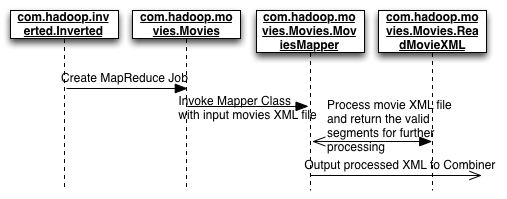
\includegraphics[width=1\textwidth]{./Figures/InvFileMap.png}
	\caption{Inverted File Mapper Sequence}
	\label{fig:invmap}
\end{figure}

\begin{figure}[H]
	\centering
	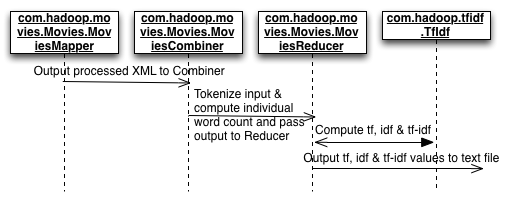
\includegraphics[width=1\textwidth]{./Figures/InvFilePrjMapCombiner.png}
	\caption{Inverted File Mapper-Combiner Sequence}
	\label{fig:invmapcombinered}
\end{figure}

\subsection{Sample Output}
At the end of the tf-idf calculation process, a tab-delimited text file is created in the 'result' directory of the project that shows the word, the number of times it has occurred within the document (count) and the tf, idf and tf-idf values for that word in a tab-delimited file. Figure \ref{fig:idfsnip} below show a snippet of the sample output file generated using the \textit{movies.xml} database as an input.

\begin{figure}[H]
	\centering
	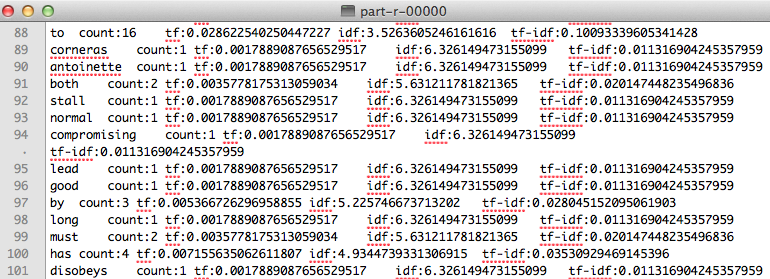
\includegraphics[width=1\textwidth]{./Figures/idfsnip.png}
	\caption{Snippet from IDF output document}
	\label{fig:idfsnip}
\end{figure}

\subsection{Analysis}
Future improvments to this application would be:
\begin{itemize}
\item Be able to accept any type of files (XML, text, etc.)
\item Better tokenization of abbreviations (Col., Lt., Dr., etc.)
\end{itemize}
\end{document}


